\documentclass[aspectratio=169,
				xcolor=table]{beamer}


\setbeamertemplate{caption}{\raggedright\insertcaption\par}


% Load general definitions
\usepackage[utf8]{inputenc}
%\usepackage[T1]{fontenc}
\usepackage[brazil]{babel}
\usepackage{amsmath}
\usepackage{amsfonts}
\usepackage{amssymb}
\usepackage{graphicx}
\usepackage{verbatim}
\usepackage{cancel}
\usepackage{askmaps}
\usepackage{tabularx}
\usepackage[table]{xcolor}
%\usepackage{tikz}
\usepackage{multirow}
\usepackage{mathtools}
\usepackage{color, colortbl}
\usepackage{etoolbox}
\usepackage{pbox}
\usepackage{changepage}
\usepackage{xpatch}
\usepackage{array}
\usepackage{marvosym}
\usepackage{tabu}
\usepackage{multicol}
\usepackage{listings}
\usepackage{underscore}
\usepackage{filecontents}
\usepackage[]{algorithm2e}
\usepackage{ragged2e}

\newcolumntype{P}[1]{>{\centering\arraybackslash}m{#1}}
\definecolor{Gray}{gray}{0.75}
\definecolor{Gray2}{gray}{0.85}

\definecolor{lightBlue}{HTML}{DAE8FC}
\definecolor{Blue}{RGB}{51, 51, 204}

%\useinnertheme[lily]{rounded}
\usetheme{UniEvangelica}
%\usetheme{Copenhagen}
%\usetheme{Berlin}
%\usecolortheme{dolphin}
\tolerance=1
\emergencystretch=\maxdimen
\hyphenpenalty=10000
\hbadness=10000

\setbeamertemplate{navigation symbols}{}%remove navigation symbols


\let\olditem=\item% 
\renewcommand{\item}{\olditem \justifying}%
\def\center{\trivlist \centering\item\relax}
\def\endcenter{\endtrivlist}

\setbeamertemplate{itemize/enumerate body begin}{\large}
\setbeamertemplate{itemize/enumerate subbody begin}{\large}

\setbeamertemplate{itemize item}{\raisebox{0.1ex}{$\blacktriangleright$}\hskip0.1em}
\setbeamertemplate{itemize subitem}{\raisebox{0.1ex}{$\blacktriangleright$}\hskip0.1em}

\newcommand{\greenarrow}{\textcolor{green}{\rotatebox[origin=c]{180}{\MVArrowDown}}}

\newcommand{\redarrow}{\textcolor{red}{\MVArrowDown}}

%\newcommand{\ftable}{
%	\begin{table}
%		\large
%		\centering
%		\rowcolors{1}{\ifnumless{\rownum}{2}{Blue}{lightBlue}}{}
%}

\newenvironment{eftable}{
	\begin{table}
		\large
		\centering
		\rowcolors{1}{}{Blue}
		\rowcolors{1}{\ifnumless{\rownum}{2}{Blue}{lightBlue}}{}
	}
	{
	\end{table}
}


%\setbeamertemplate{frametitle}
%{
%	%\vspace*{-2em}	
%	\insertframetitle
%
%	 %\textcolor{white}{\LARGE \insertframetitle}
%
%}

% Specific definitions
\institute[]{\uppercase{Engenharia de Computação}}
\title[]{Prática em Fábrica de Software III}
\subtitle[]{\uppercase{Teoria de Sinais}}
\author[]{Prof. M.e Alexandre Tannus}
\date{Anápolis - 2019.2}

%\AtBeginSection{\frame{\tableofcontents[currentsection]}}

\begin{document}
	\begin{frame}
		\titlepage		
	\end{frame}

	\begin{frame}
		\tableofcontents
	\end{frame}	

	\section{Introdução}
	\begin{frame}{Introdução}
		\begin{itemize}
			\item Sinal
			\begin{itemize}
				\item Função que representa uma variável física e contém a informação sobre a dinâmica de um dado fenômeno
			\end{itemize}
		\end{itemize}
		
		\begin{figure}[hbtp]
		\centering
		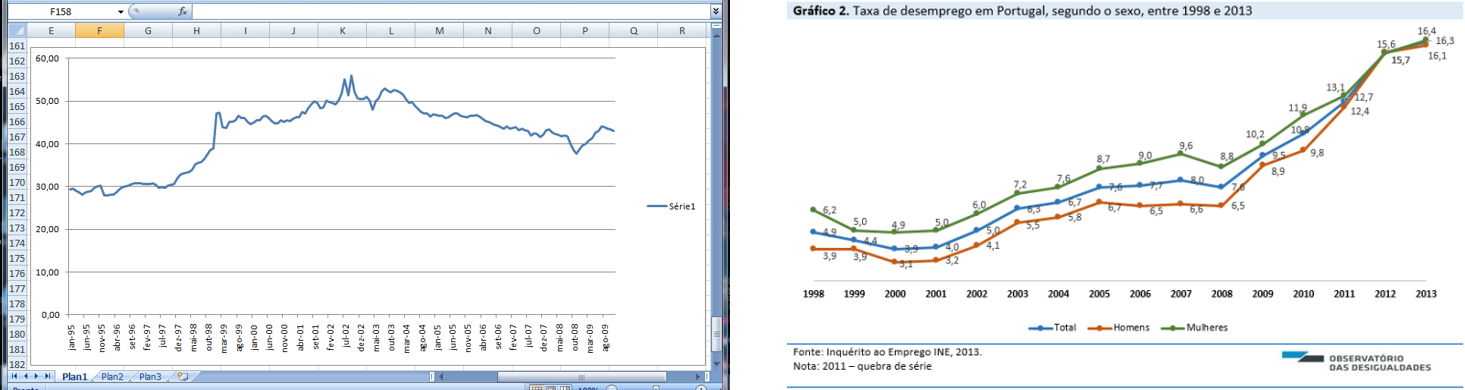
\includegraphics[width=0.8\textwidth, keepaspectratio]{../figs/cap01/sinal01.png}
		\end{figure}
		
	\end{frame}
	
		\begin{frame}{Introdução}
		
		\begin{figure}[hbtp]
		\centering
		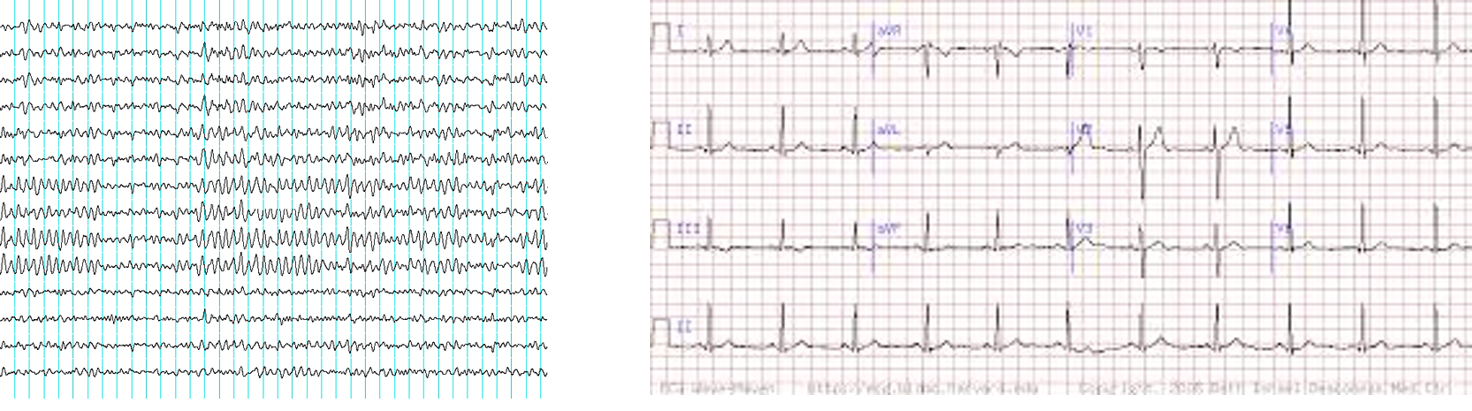
\includegraphics[width=0.95\textwidth, keepaspectratio]{../figs/cap01/sinal02.png}
		\end{figure}
		
	\end{frame}
	
	\begin{frame}{Por que processar sinais?}

		\begin{itemize}
			\item Remoção de ruído
			\vspace{.7em}
			\item Extração de características de interesse
			\vspace{.7em}
			\item Classificação
			\vspace{.7em}
			\item Encontrar relações de entrada/saída
			\vspace{.7em}
			\item Compressão de dados
			\vspace{.7em}
			\item Predição de valores futuros
		\end{itemize}	
		
	\end{frame}


	\section{Classificação dos sinais}	
	
	\begin{frame}{Classificação de Sinais}
		\begin{itemize}
			\item Contínuos vs Discretos no tempo
			\vspace{1em}
			\item Analógicos vs Digitais
			\vspace{1em}
			\item Determinísticos vs aleatórios
			\vspace{1em}
			\item Periódicos vs não-periódicos
			\vspace{1em}
		\end{itemize}		
	\end{frame}
	
	\begin{frame}{Sinal Contínuo vs Discreto no tempo}
		\begin{itemize}
			\item Contínuo 
			\begin{itemize}
				\item definidos para valores contínuos de tempo.
				\item Exemplo: temperatura
			\end{itemize}
			\vspace{1em}
			\item Discreto
			\begin{itemize}
				\item definidos para valores discretos de tempo. 
				\item Exemplo: cotação diária de uma determinada ação
			\end{itemize}
		\end{itemize}
	\end{frame}
	
	\begin{frame}{Sinal Analógico vs Digital}
		\begin{itemize}
			\item Analógico
			\begin{itemize}
				\item amplitude pode assumir valor dentro de uma faixa contínua.
			\end{itemize}
			\vspace{1em}		
			\item Digital
			\begin{itemize}
				\item amplitude pode assumir M valores dentro de uma faixa de
amplitudes (sinal M-ário).
			\end{itemize} 
		\end{itemize}		
	\end{frame}
	
	\begin{frame}{}
				
		\begin{figure}[hbtp]
			\centering
			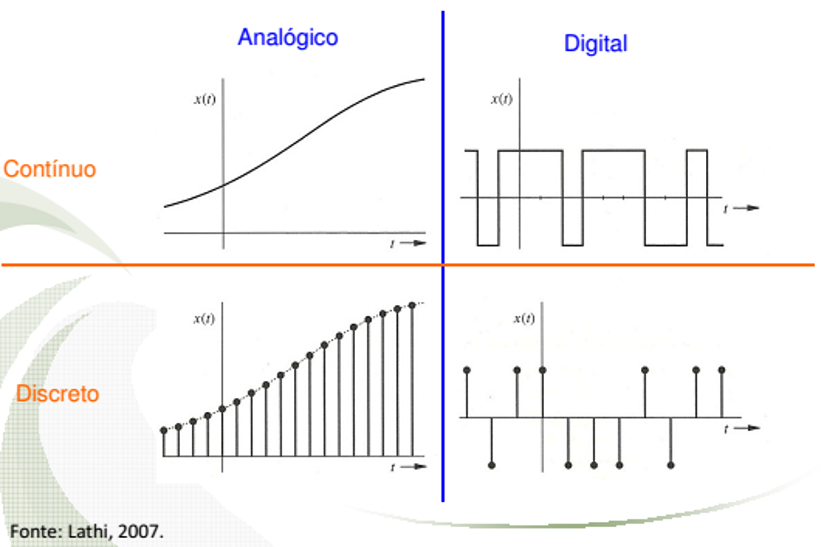
\includegraphics[width=0.7\textwidth, keepaspectratio]{../figs/cap01/sinais.png}
		\end{figure}
	\end{frame}
	
	\begin{frame}{Sinal Determinístico vs Aleatório}
	
		\begin{itemize}
			\item Determinístico
			\begin{itemize}
				\item Pode ser completamente descrito por uma equação ou fórmula matemática
				\item Exemplo: $x(t)=X\sin(2 \pi f_0 t + \Theta)$
			\end{itemize}				
			\begin{figure}[hbtp]
				\centering
				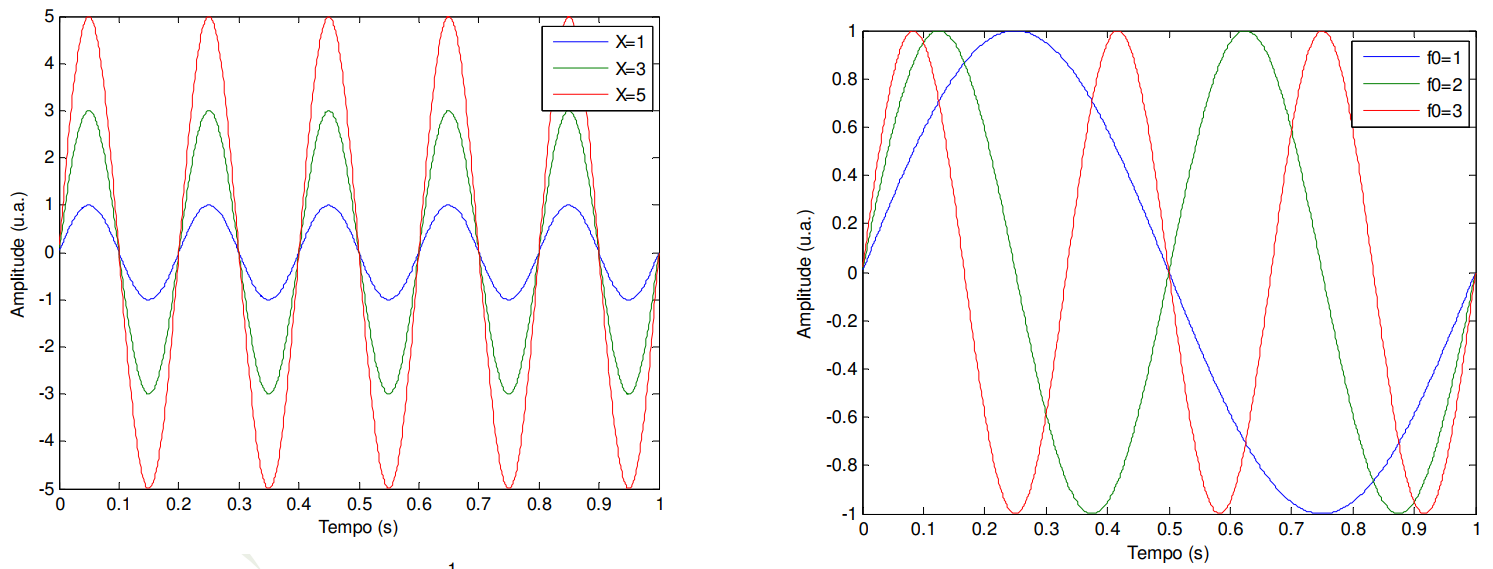
\includegraphics[width=0.7\textwidth, keepaspectratio]{../figs/cap01/deterministico.png}
			\end{figure}		
		\end{itemize}
		
	\end{frame}
	
	\begin{frame}{Sinal Determinístico vs Aleatório}
		\begin{itemize}
			\item Aleatório
			\begin{itemize}
				\item Somente pode ser descrito por uma distribuição probabilística ou seus parâmetros (e.g.: valor médio, variância)
			\end{itemize}
		\end{itemize}
		
		\begin{columns}
			\begin{column}{0.5\textwidth}
				\begin{figure}[hbtp]
					\centering
					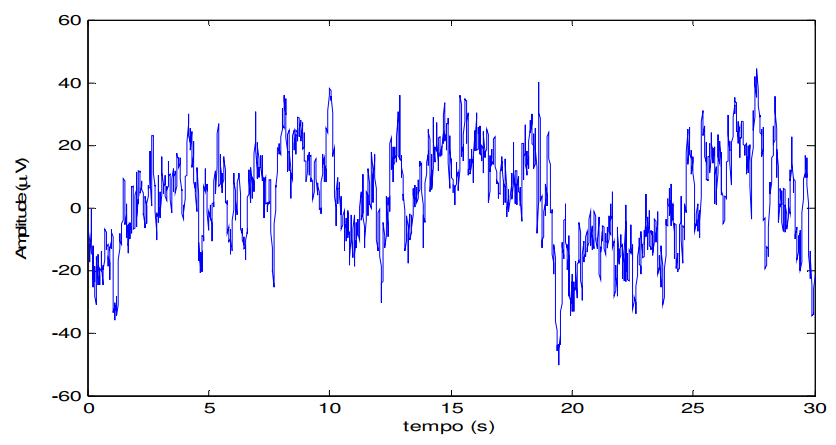
\includegraphics[width=0.9\textwidth, keepaspectratio]{../figs/cap01/aleatorio01.png}
				\end{figure}
			\end{column}
			\begin{column}{0.5\textwidth}
				\begin{figure}[hbtp]
					\centering
					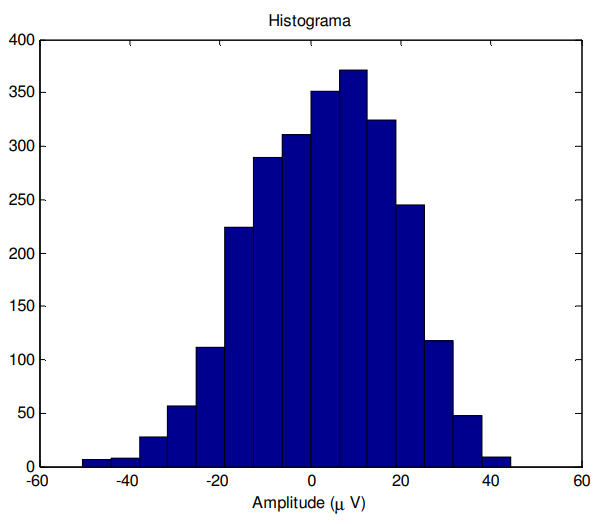
\includegraphics[width=0.8\textwidth, keepaspectratio]{../figs/cap01/aleatorio02.png}
				\end{figure}
				
			\end{column}
		\end{columns}
	\end{frame}
	
	
	\section{Sistema de Aquisição de Sinais}
	\begin{frame}{Sistema de Aquisição de Sinais}
		
		\begin{figure}[hbtp]
			\centering
			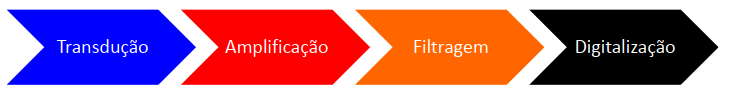
\includegraphics[width=\textwidth, keepaspectratio]{../figs/cap01/sistema01.png}
		\end{figure}		
		
		\begin{itemize}
			\item \textcolor{blue}{Conversão de uma grandeza física em outra (usualmente tensão ou corrente)}
			\item \textcolor{red}{Aplicação de um fator de Ganho}
			\item \textcolor{orange}{Remoção de freqüências que não são de interesse}
			\item  Passagem do domínio contínuo para o discreto
		\end{itemize}
		
	\end{frame}
	
	\begin{frame}{Aquisição de Sinais}
		
		\begin{figure}[hbtp]
			\centering
			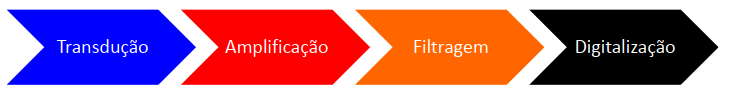
\includegraphics[width=\textwidth, keepaspectratio]{../figs/cap01/sistema01.png}
		\end{figure}	
		
		\textcolor{blue}{Conversão de uma grandeza física em outra (usualmente tensão ou corrente)}
		
		\begin{figure}[hbtp]
			\centering
			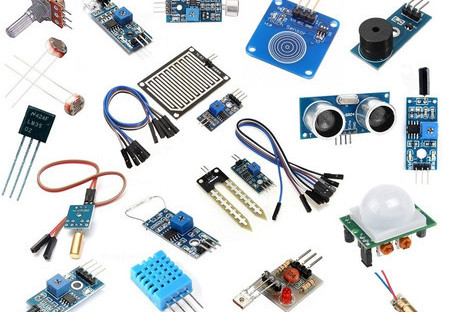
\includegraphics[height=0.4\textheight, keepaspectratio]{../figs/cap01/transdutores}
		\end{figure}	
					
	\end{frame}
	
	\begin{frame}{Amplificação}
		
		\begin{figure}[hbtp]
			\centering
			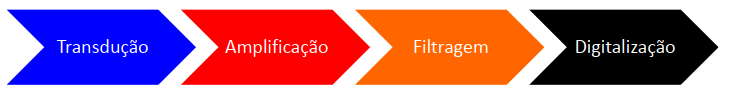
\includegraphics[width=\textwidth, keepaspectratio]{../figs/cap01/sistema01.png}
		\end{figure}	
		
		\textcolor{red}{Aplicação de um fator de Ganho}
		
		\vspace{-3em}
		\begin{columns}
			\begin{column}{0.25\textwidth}
				\begin{figure}[hbtp]
					\centering
					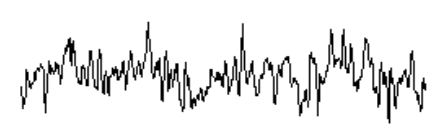
\includegraphics[width=\textwidth, keepaspectratio]{../figs/cap01/sinalori.png}
				\end{figure}	
				
			\end{column}
			\begin{column}{0.25\textwidth}
				\begin{figure}[hbtp]
					\centering
					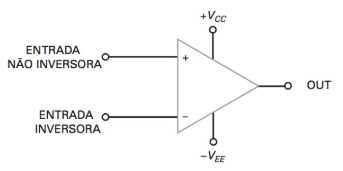
\includegraphics[width=\textwidth, keepaspectratio]{../figs/cap01/ampop.png}
				\end{figure}	
				
			\end{column}
			\begin{column}{0.4\textwidth}
				\begin{figure}[hbtp]
					\centering
					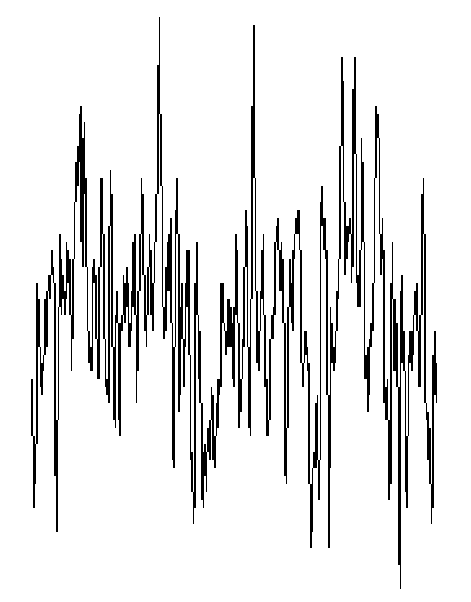
\includegraphics[width=.7\textwidth, keepaspectratio]{../figs/cap01/sinalamp.png}
				\end{figure}	
				
			\end{column}
		\end{columns}
	
	\end{frame}
	
	\begin{frame}{Filtragem}
		
		\begin{figure}[hbtp]
			\centering
			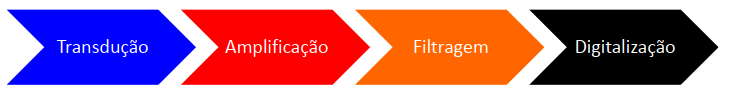
\includegraphics[width=\textwidth, keepaspectratio]{../figs/cap01/sistema01.png}
		\end{figure}	
		
		\textcolor{orange}{Remoção de freqüências que não são de interesse}
		
		\begin{figure}[hbtp]
			\centering
			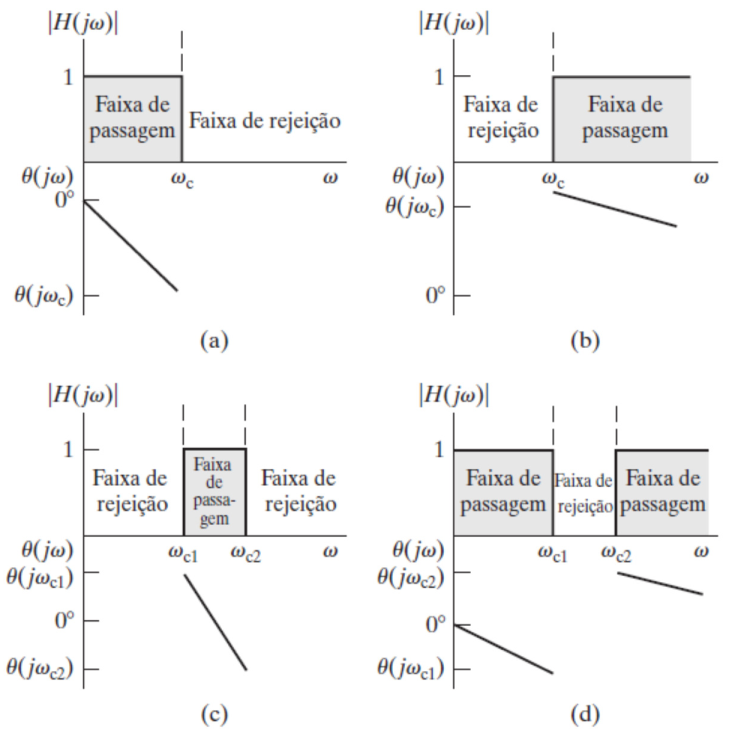
\includegraphics[height=4cm, keepaspectratio]{../figs/cap01/filtro.png}
		\end{figure}	
		
	\end{frame}
	
	\begin{frame}{Digitalização}
		\begin{figure}[hbtp]
			\centering
			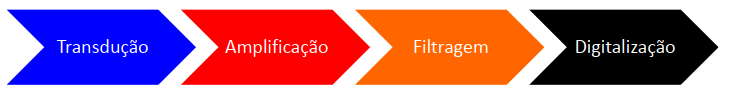
\includegraphics[width=\textwidth, keepaspectratio]{../figs/cap01/sistema01.png}
		\end{figure}	
		
		Passagem do domínio contínuo para o discreto e quantização.
				
		\begin{figure}[hbtp]
			\centering
			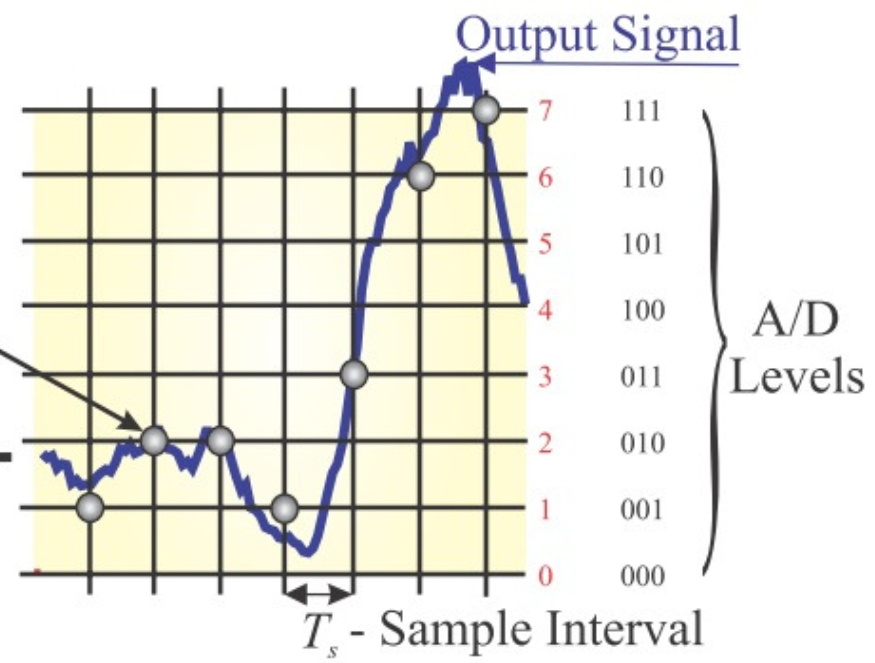
\includegraphics[width=.25\textwidth, keepaspectratio]{../figs/cap01/ad01.png}
		\end{figure}	
		
		Características importantes: faixa de entrada, resolução, taxa máxima de amostragem
	\end{frame}	
	
	
	\section{Conversão Analógico-Digital (A/D)}
	
	\begin{frame}{Conversor A/D - Amostragem}	
		\begin{figure}[hbtp]
			\centering
			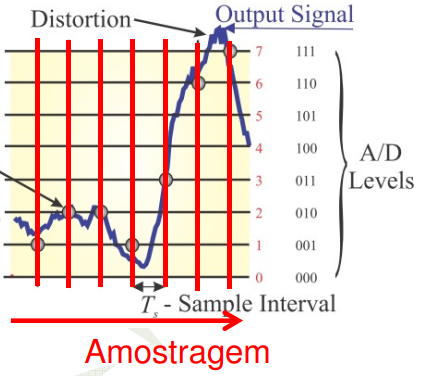
\includegraphics[width=.35\textwidth, keepaspectratio]{../figs/cap01/ad02.png}
		\end{figure}
	\end{frame}
	
	\begin{frame}{Amostragem - Teorema de Nyquist}
		\vspace{-2em}	
		\begin{columns}[t]
			\begin{column}{0.25\textwidth}	
				\begin{figure}[hbtp]
					\centering
					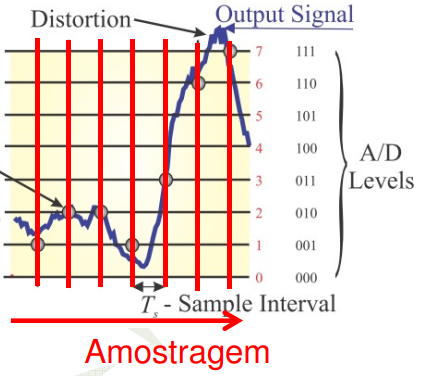
\includegraphics[width=\textwidth, keepaspectratio]{../figs/cap01/ad02.png}
				\end{figure}
				
			\end{column}
			\begin{column}{0.7\textwidth}	
		\begin{figure}[hbtp]
			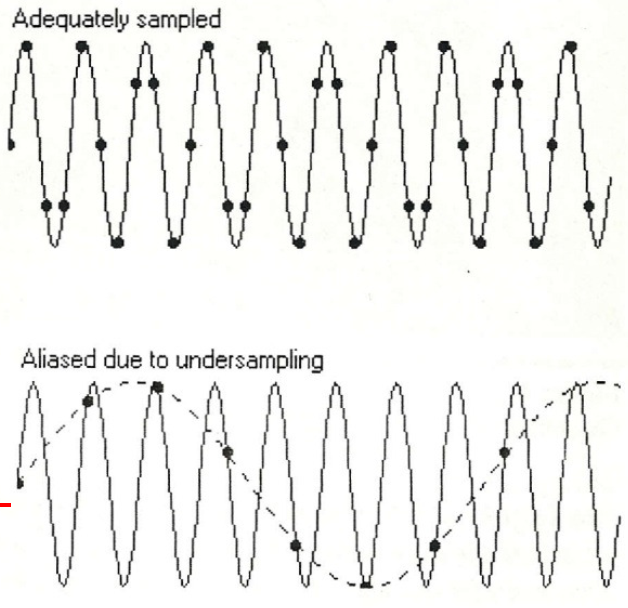
\includegraphics[width=.7\textwidth, keepaspectratio]{../figs/cap01/nyquist.png}
		\end{figure}
				
			\end{column}
		\end{columns}
	\end{frame}
	
	\begin{frame}{Conversor A/D - Faixa de entrada}
		\begin{itemize}
			\item Corresponde à faixa de amplitude que possui representação no conversor A/D.
		\end{itemize}
		\begin{figure}[hbtp]
			\centering
			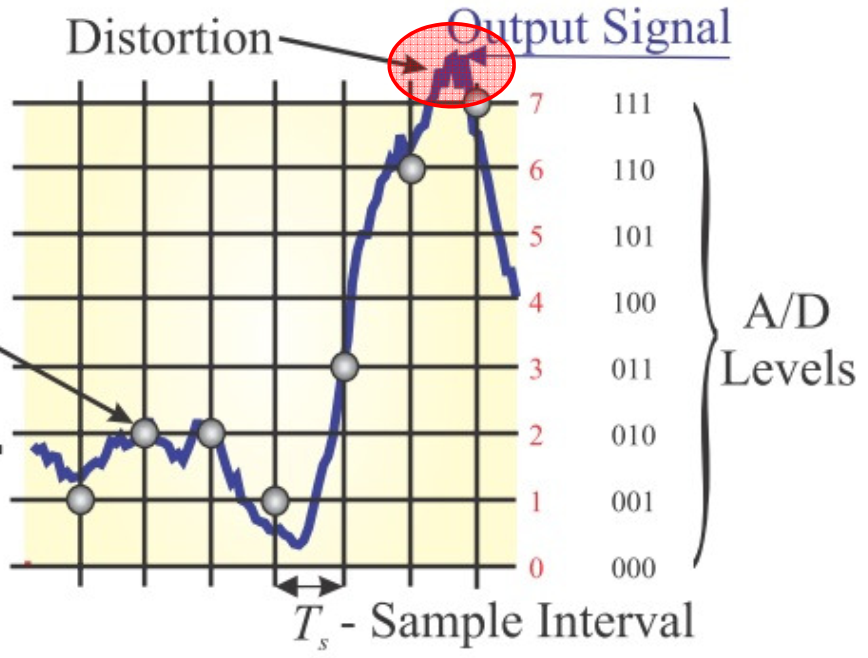
\includegraphics[height=.65\textheight, keepaspectratio]{../figs/cap01/ad04.png}
		\end{figure}
	\end{frame}
	
	\begin{frame}{Conversor A/D - Resolução}
		\begin{itemize}
			\item Corresponde ao número de bits utilizados para representar valores de amplitude do sinal.
		\end{itemize}
		\vspace{-1.5em}
		\begin{columns}
			\begin{column}{0.5\textwidth}
				\begin{figure}[hbtp]
					\centering
					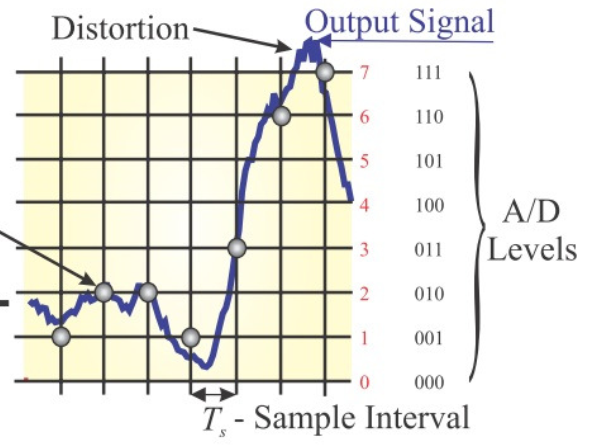
\includegraphics[height=.6\textheight, keepaspectratio]{../figs/cap01/res3bits.png}
					\caption{Resolução: 3 bits}
				\end{figure}
			\end{column}
			\begin{column}{0.5\textwidth}
				\begin{figure}[hbtp]
					\centering
					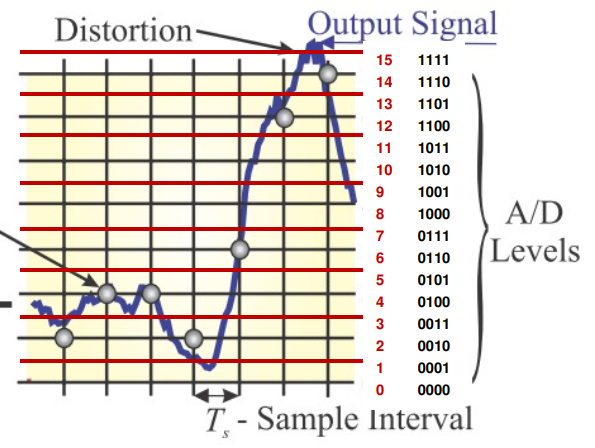
\includegraphics[height=.6\textheight, keepaspectratio]{../figs/cap01/res4bits.png}
					\caption{Resolução: 4 bits}
				\end{figure}
			\end{column}
		\end{columns}
	\end{frame}

	\begin{frame}{Exemplo}
	
		\begin{block}{}
			\textbf{Amplificador com Ganho:} $A=10000$
			
			\textbf{Conversor A/D:} $b=8 bits$
			
			\textbf{Faixa de entrada do Conversor A/D:} $V_{max}=5V$
		
		\end{block}
		\begin{itemize}
				\item Qual a faixa de entrada do sistema de aquisição? %Vmax/A=5/10000=500µV
				\item Quantos níveis tem este conversor A/D? %2b=28=256
				\item Qual a resolução na entrada? %500µV/256=1,95µV
		\end{itemize}
		
	\end{frame}
	

	\begin{frame}{Exemplo}
	
		\begin{block}{}
			\textbf{Amplificador com Ganho:} $A=10000$
			
			\textbf{Conversor A/D:} $b=8 bits$
			
			\textbf{Faixa de entrada do Conversor A/D:} $V_{max}=5V$
		
		\end{block}
		
			
			\begin{itemize}
				\item Qual a faixa de entrada do sistema de aquisição? 
				\pause
				\begin{itemize}
					\item $\frac{V_{max}}{A}=\frac{5}{10000}=500\mu V$
				\end{itemize}
				\pause
				\item Quantos níveis tem este conversor A/D? 
				\pause
				\begin{itemize}
					\item $2^b=2^8=256$
				\end{itemize}
				\pause
				\item Qual a resolução na entrada? 
				\pause
				\begin{itemize}
					\item $\frac{500 \mu V}{256}=1,95 \mu V$
				\end{itemize}
			\end{itemize}
	\end{frame}
		
	\begin{frame}{}
	\end{frame}	
\end{document}
